\documentclass{article}
\usepackage[utf8]{inputenc}
\usepackage{amsmath}
\usepackage{graphicx}
\usepackage[margin=1.5in]{geometry}

\title{Assistentenhandleiding biomechanica}
\author{Munib Özdemir}
\date{juli 2022}

\begin{document}

\maketitle

\section{Introductie}
Deze handleiding zal de belangrijkste aspecten van het experiment (bio)mechanica bespreken om de assistent zo goed mogelijk voor te bereiden. Dit is een relatief open experiment, omdat we niet alleen biomechanica maar ook klassieke mechanica experimenten zullen tegenkomen. In deze handleiding zullen we daarom meer focus leggen op het voorbereiden en uitvoeren van biomechanica experimenten. Aanvullingen of verbeteringen zijn welkom!
\\\\

\section{Hardware en software}
\subsection{Hardware}
De apparatuur en software die we tijdens dit experiment zullen gebruiken worden hier kort besproken, evenals aanvullende informatie die nuttig kan zijn voor studenten en assistenten en extra intuïtie kan bieden. Een completere uitleg van de hardware en software is te vinden in de handleiding. Voor de experimenten maken we gebruik van een  hogesnelheidscamera die met maximaal 700 fps (frames per second, beelden per seconde) kan opnemen. Voor veel studenten die geen of weinig ervaring hebben met camera's of fotografie, zullen termen zoals frame rate, shutter (sluiter), exposure time (sluitertijd) etc. nieuw zijn. De assistent zal dan niet alleen uit moeten leggen wat deze termen betekenen, maar ook hoe deze termen in de praktijk uitpakken. \\\\ Verder maken we gebruik van LED lichtjes die we kunnen plaatsen of kunnen ophangen op het lichaam. Hiernaast hebben we ook theaterlampen ter beschikking om objecten mee te belichten. Door de korte sluitertijd ($\sim$1ms), is het beeld wat we verkrijgen met de camera erg donker, hierdoor is licht erg nuttig want het zorgt voor extra belichting van de sensor. De theaterlampen zijn erg fel en kunnen erg warm worden, dus probeer niet direct in het licht te kijken of het koellichaam op de achterkant aan te raken! Meestal worden LED lichtjes gebruikt voor biomechanica experimenten, zoals markers die bij scharnierpunten worden geplaatst. theaterlampen zijn meestal niet geschikt voor zulke experimenten, omdat de software die wij gebruiken een hoog contrast nodig heeft om objecten (in dit geval scharnierpunten) te kunnen volgen. \\\\ Om de camera te monteren en positioneren gebruiken we een camera beugel. Deze zal vooral handig zijn omdat de beeldverhouding van de camera ongeveer 1.88:1 is (het beeld is 1,88 keer zo lang dan het breed is), waardoor we processen die vooral in de hoogte afspelen, zoals het vallen van een object, goed in beeld kunnen brengen. Dit kunnen we doen door de camera 90 graden te draaien, waardoor de beeldverhouding 1:1.88 wordt. \\\\ Om een scherp beeld te krijgen gebruiken we een lens. Studenten zullen over het algemeen met trail and error wel een scherp beeld krijgen, maar hebben meestal geen kennis over het instellen van een lens. In de handleiding staat kort uitgelegd wat de functie van elke tussenring (ringen waar je aan kan draaien) is, maar belangrijk is dat de ring het dichtst bij de camera (aperture ring of sluiterring) zo ver mogelijk open staat. Dit om zoveel mogelijk licht binnen te laten vanwege de lage sluitertijd. Dit heeft wel het gevolg dat objecten relatief snel focus verliezen als ze naar of van de camera af bewegen (depth of field, scherptediepte). De andere twee ringen, de focus en zoom, worden door de studenten intuïtief ingesteld.

\subsection{Software}
Voor de software voor dit experiment gebruiken we drie programma's:
\begin{itemize}
\item \textbf{LuCam Capture}. Over het algemeen gebruiken we LuCam Capture alleen om de camera te testen, met LuCam Capture kan er er alleen foto's vastgelegd wroden en kan geen filmpjes mee worden opgenomen. Toch is het erg handig te zien hoe de instellingen het beeld veranderen. 
\item \textbf{TroublePix}. Om beelden op te nemen gebruiken we TroublePix. De instellingen bij LuCam Capture zijn ook te vinden bij TroublePix, al is het af en toe iets lastiger om deze te vinden.
\item \textbf{MaxTRAQ}. Als laatste gebruiken we ook nog MaxTRAQ, dit is een motion capture programma, wat inhoudt dat je met behulp van dit programma bijvoorbeeld de positie van objecten, hoeken tussen objecten en afstanden kunt tracken. Dit wordt gedaan met behulp van trackers. De gebruiker kiest een punt die getracked wordt, dit is meestal een object met een hoog contrast zoals een wit plakkertje, en zolang het programma het punt herkent wordt deze frame per frame gevolgd. Tracking wordt gedaan door in het begin een pixel of groep van pixels als referentie pixels te nemen, en deze binnen een kader van frame tot frame te volgen. Soms mislukt tracken omdat zich binnen dat kader een soortgelijke groep pixels bevindt of als de vorm van de marker te veel verandert. Hiervoor zijn er een aantal oplossingen voor: MaxTRAQ pauzeert de video tijdens het tracken wanneer dit mislukt. De pixels kunnen dan handmatig worden gekozen totdat het tracken weer door MaxTRAQ gedaan kan worden. Let wel op dat dit handig is voor een paar frames, anders zal het tracken veel tijd kosten. Als het tracken mislukt voor een lang tijdsinterval (tientallen tot honderden frames) is het handig om te kijken hoe goed het object zichtbaar is. Als het object zichtbaar is, maar er zijn soortgelijke belichte objecten in de buurt dan is het handig om het zoekvenster van MaxTRAQ aan te passen. In het ergste geval moet het filmpje nog een keer opgenomen worden. Het is dan verstandig om te kijken of de region of interest (ROI) aangepast kan worden om alleen het object zichtbaar te maken.
\end{itemize}
\section{Indeling dagdelen}
\subsection{Dagdeel 1 (Verkenning)}
Tijdens dit dagdeel wordt de basis gelegd voor de hardware en software door deze te verkennen en introducerende experimenten uit te voeren. Meestal begint de assistent dit dagdeel met een presentatie of een korte introductie over wat het experiment (bio)mechanica inhoudt. Er kan voor gekozen worden om de verkenning van de camera en driver (sectie 2 in de handleiding) samen te doen of de student dit zelfstandig te laten lezen. 
\subsubsection{Opdracht 1}
Tijdens dit deel moet worden gekeken naar de camera, lens en het programma LuCam Capture. Bij opdracht 1 is het de bedoeling de student kennis te laten maken met de camera, beugel en software. Ook wordt met behulp van een kalibratiepaneel het beeld gekalibreerd. Het paneel wordt belicht met theaterlampen om zo de zoom en focus goed in te stellen. Er wordt als laatste gevraagd naar de kleinste en grootste afstand vanaf de camera waar het paneel nog goed in focus is. Theoretisch gezien is het lastig om te bepalen wat 'goed in focus' is, omdat dit afhangt van meerdere factoren. De depth of field wordt gegeven door,
\begin{align*}
DoF \approx \frac{2u^2Nc}{f^2}
\end{align*}
waarbij $u$ de afstand tot het object, $N$ de $f$-number, $f$ de focal length en $c$ de circle of confusion. De circle of confusion hangt af van een aantal variabelen: de grootte van sensor, hoe groot het uitendelijke plaatje wordt afgebeeld enz. We nemen voor nu een circle of concfusion van $c=0.008$mm aan. Zie figuur \ref{fig:dof} voor hoe de verschillende factoren zich met elkaar verhouden.\\ Laten we een voorbeeld doen: Het kalibratiepaneel staat op een afstand van 2m. We proberen altijd een zo groot mogelijke sluiter (aperture) te gebruiken, in dit geval $f/1.4 \to N=1.4$. De circle of confusion was eerder gegeven $c=0.008$. Voor de focal length nemen we de kleinste focal length (dus zo ver mogelijk uitgezoomd), $f=11.5$mm. Dit geeft ons een $DoF\approx 677$mm. De kleinste afstand die nog goed in focus is, is dan $DoF_{\text{near limit}}=u-\frac{DoF}{2}=1.662$m en de grootste afstand is $DoF_{\text{far limit}}=u+\frac{DoF}{2}=2.339$m. Merk op dat de depth of field schaalt als het kwadraat van de afstand $DoF \sim u^2$, dus een kleinere afstand kiezen kan de depth of field significant verminderen.
De ondergrens van de focus van de lens ligt rond een meter, en in principe zit er geen bovengrens aan de grootste afstand. Let wel op dat de nauwkeurigheid van de data onder andere afhankelijk is van de afstand tot het object, dus dit betekent dat je de camera zo dicht mogelijk wilt hebben. De uitdaging bij deze opdracht is het bepalen van de juiste focus. Dit kan lastig zijn maar belangrijk is om te zien of de grens tussen witte en zwarte vlakken niet wazig is. Door de depth of field is er een bereik aan focussen die 'goed' zijn, en meestal lijdt de kwaliteit er niet veel onder zolang het object binnen dit bereik ligt. Om vertekening van de beelden te voorkomen moet de voorkant van de lens goed parallel staan aan het objectvlak en dient de camera goed horizontaal of verticaal te staan.

\begin{figure}
    \centering
    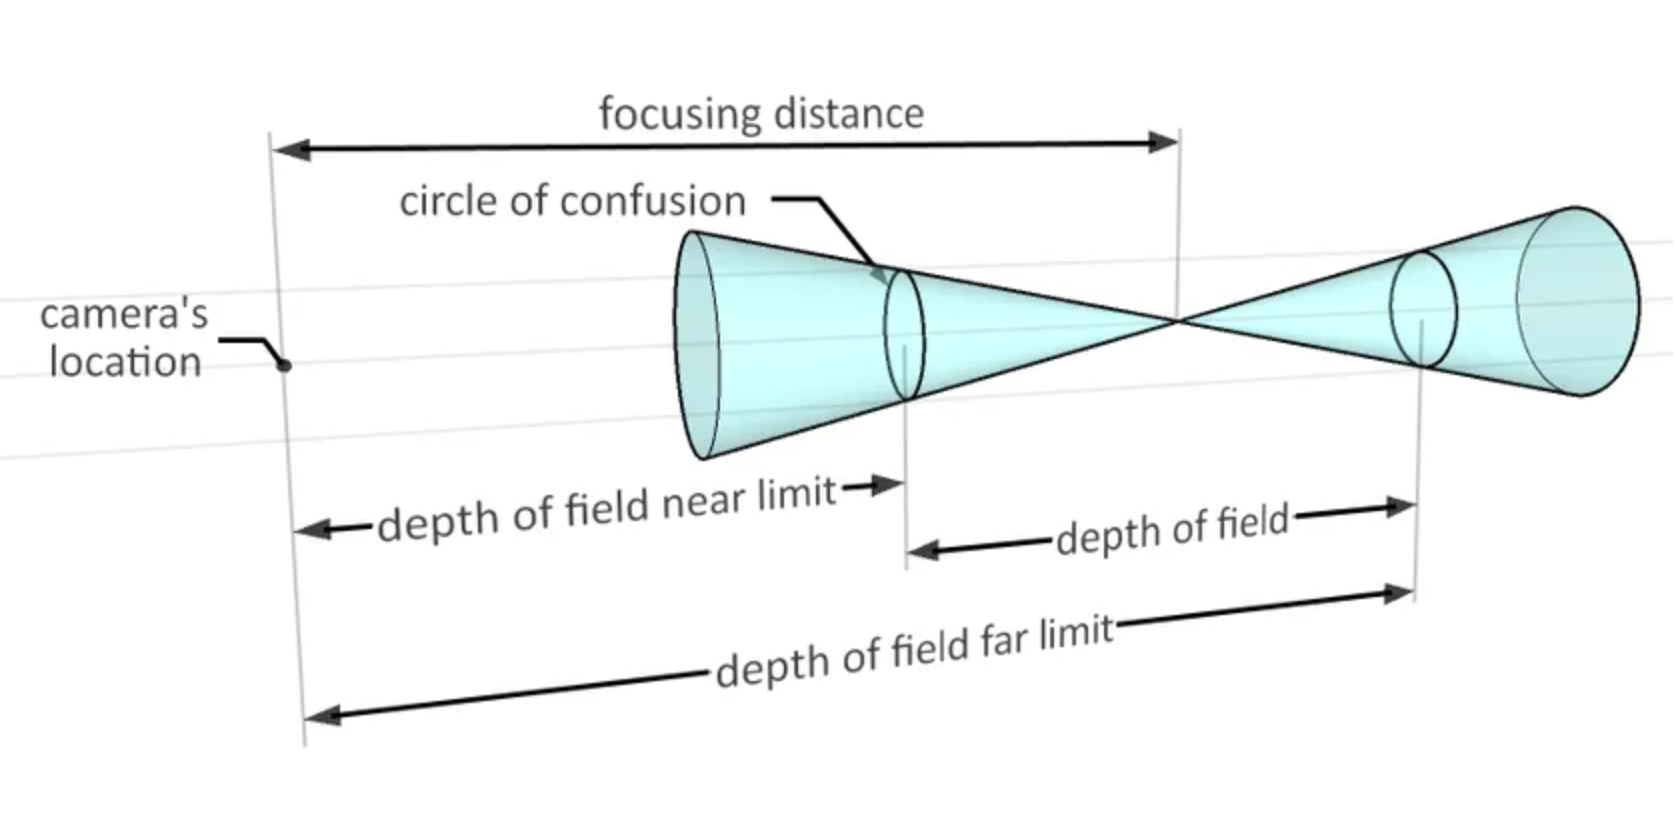
\includegraphics[width=\textwidth]{figures/dof.png}
    \caption{Afgebeeld hoe lichtstralen vanaf de focus lopen. Hier is ook te zien hoe de depth of field afhangt van de circle of confusion. Een grotere circle of confusion betekent meestal ook een grotere depth of field.}
    \label{fig:dof}
\end{figure}

\subsubsection{Opdracht 2}
In deze opdracht wordt de software verkend en starten we eerst met TroublePix. Dit wordt uitgebreid in de handleiding uitgelegd en er kan hier weer gekozen worden om de student dit zelfstandig te laten lezen, of anders de video op Canvas te laten bekijken (er is nog geen video bij het schrijven van deze handleiding). Hierna volgt opdracht 2, in deze opdracht wordt de student aan het denken gezet over de bandbreedte tijdens het filmen. De bandbreedte (informatie per seconde, in dit geval bits of bytes per seconde) wordt gegeven door
\begin{equation}\label{eq:1}
    \text{bandwidth} = \text{resolution} \times \text{frame rate} \times \text{color depth}
\end{equation}
waarbij de resolution wordt berekend door het product van de verticale en horizontale pixels. Color depth, of kleurendiepte, is een maat voor de hoeveelheid kleuren die een pixel kan aannemen. Voor dit experiment wordt er 8-bit grayscale gebruikt (8-bit zwart-wit), wat betekent dat er $2^8=256$ zwart-wit tinten beschikbaar zijn. We zullen tijdens dit experiment zwart-wit gebruiken omdat kleur (in TroublePix 12-bit) in de meeste gevallen geen toegevoegde waarde heeft. De bandbreedte wordt ook gelimiteerd door de gebruikte dataverbinding, in ons geval het USB 3.0 protocol. Een voorbeeld voor USB 3.0: De maximale theoretische overdrachtssnelheid die USB 3.0 kan leveren is 5 Gbps (5 Gigabit per seconde = 625 MegaByte per seconde, b = bit en B = Byte). Als we dit vergelijken met de bandbreedte van de video met de best mogelijke (maximale resolutie, beste kleurendiepte en hoogste frame rate) die de camera kan leveren komen we uit op een bandbreedte van $2048 \times 1088 \times 170 \times 12 = 4,55$ Gbps = 568,75 MBps. \\Dit betekent dat een filmpje van een aantal seconde al snel gigabytes aan opslag kan vullen. Omdat we de kleurendiepte constant houden is de bandbreedte een strijd tussen de resolutie en de frame rate, dus als je bijvoorbeeld een filmpje wilt opnemen met een hogere frame rate moet je een lagere resolutie nemen. Een andere resolutie kiezen kan je op twee manieren doen: je kan uit de lijst van resoluties de kiezen of je kan de Region Of Interest (ROI) aanpassen, waardoor je in principe een custom resolutie maakt. Bij opdracht (a) wordt er gevraagd naar de maximale frame rate bij maximale resolutie, dit is voor 8-bit ongeveer 250 fps. De student zal hierachter moeten komen door daadwerkelijk het filmpje te maken, omdat de berekeningen die we hier doen kunnen afwijken van de praktijk. Het is mogelijk dat de frame rate significant kan afwijken (in de tientallen procenten) als de camera erg warm is of als de camera is aangesloten aan een USB 2.0 poort. De camera kan in portrait (langer verticaal dan horizontaal) en landscape (langer horizontaal dan verticaal) worden gepositioneerd. Voor een object wat valt is het handiger om het in portrait te zetten, omdat de beweging van een vallend object alleen maar in de hoogte (dus verticaal) gebeurt. Bij (c) wordt er gevraagd hoe we nog een hogere frame rate kunnen halen. Zoals eerder genoemd is de bandbreedte afhankelijk van de frame rate en resolutie. Omdat we werken met de maximale resolutie, kunnen we een kleinere resolutie nemen en hiervan de ROI aanpassen om zo een hogere frame rate te krijgen.

\subsubsection{Opdracht 3}
Dit is de eerste opdracht waarbij alle kennis over hardware en software wordt toegepast bij een experiment. De studenten zullen met deze opdracht de valversnelling $g$ bepalen met behulp van een slinger. Hiervoor gebruiken we een model van een simpele harmonische oscillator, in plaats van een gedempte oscillator (kan alsnog gebruikt worden als verdiepende opdracht). De reden dat we geen gedempte oscillator gebruiken is omdat het filmpje wat wordt opgenomen maar een paar oscillaties zal bevatten. Bij (a) wordt er gevraagd waarom we de luchtweerstand kunnen verwaarlozen en als hint wordt gegeven dat de luchtweerstand evenredig is met het kwadraat van de snelheid. We mogen dit doen om twee redenen: als eerste, we kijken maar naar een paar oscillaties, dus dat betekent dat de amplitude van ons signaal nauwelijks afneemt over deze tijd. Als tweede, we mogen luchtweerstand verwaarlozen voor dezelfde reden dat ons model evenredig is aan een sinus, want we kijken naar kleine hoeken waar de snelheid relatief klein is. Nu is het aan de student om de opstelling te bouwen en de meting te doen. Als het goed is staat de camera al klaar en moet alleen de slinger klaargezet worden. De slinger zelf kan belicht worden met theaterlampen of er kan een LED lichtje worden opgehangen. Vervolgens moeten de studenten met TroublePix de best mogelijke instellingen vinden om uiteindelijk een frame rate van ongeveer 300 fps te behalen. De makkelijkste instelling is de sluitertijd, die mag maximaal $\frac{1}{300}$s zijn. Vervolgens kan je met de hoogste resolutie en juiste ROI kijken of je 300 fps kan bereiken, zo niet pas dan eerst de resolutie en dan de ROI aan. Bij het bouwen van de opstelling moet goed gelet worden op een aantal dingen:
\begin{itemize}
    \item Zorg ervoor dat de camera loodrecht staat op het vlak waarin de slinger oscilleert, als dit niet het geval is zal de beweging niet mooi sinusoidaal lijken te zijn in de video.
    \item Ook moet gelet worden op dat de camera niet te ver naast of boven de slinger staat
    \item Als het aangrijppunt niet 'perfect' is krijg je een variabele lengte van de slinger wat invloed heeft op de bepaalde waarde van $g$.
    \item Ook zal de waarde afwijken als de lengte van de slinger onjuist is bepaald.
\end{itemize}
Dit zijn tevens ook een van de redenen dat de theoretische waarde kan afwijken van de experimentele waarde. We zoeken bij (c) vooral naar het onjuist positioneren van de camera. \\\\ Voordat we opdracht 4 gaan bespreken, kijken we even kort naar biomechanica. Bijna alle assistenten zijn niet of nauwelijks in aanraking gekomen met biomechanica (als we uitgaan van natuurkunde/wiskunde en vaak zelfs MNW studenten), daarom is het handig als we hier kort bespreken hoe we moeten denken als een bewegingswetenschapper. \\\\ We zijn bij natuurkundepractica gewend om de modellen vrij makkelijk te vinden. De experimenten die we dan uitvoeren is in termen van deze theorie of modellen, waarbij we vaak de mogelijkheid hebben om een parameter continu te variëren (zoals bijvoorbeeld de massa of lengte van een slinger, druk binnen in een bal, temperatuur van een object etc.), de meting uit te voeren om data te verkrijgen en met behulp van de theorie een fit doen. Wat we moeten aannemen bij zulke experimenten is dat als we een parameter variëren de rest van de opstelling niet significant (niet genoeg om dit terug te zien in de data) verandert. Bij biomechanische experimenten is dit veel minder het geval, omdat de opstelling nu onze lichamen zijn. Dus elke keer als we een experiment uitvoeren, zoals het schoppen van een bal, zal de beweging die we uitvoeren niet twee keer hetzelfde zijn. Dit betekent dat we het experiment heel vaak over moeten doen, wat leidt tot vermoeidheid en weer andere resultaten. En dan hebben we heel vaak geen theorie waar we onze resultaten mee kunnen analyseren of kunnen vergelijken. We moeten dus onze manier van denken veranderen. In plaats van te denken in termen van variabelen die we continu kunnen veranderen, moeten we denken in termen van discrete parameters die we uit specifieke bewegingen kunnen verkrijgen. Als we de beweging uit opgave 4 nemen als voorbeeld, een schop, denken we bijvoorbeeld aan de maximale kracht die bepaalde spieren of spiergroepen uitvoeren, of de maximale torque (koppel) rond de heup, knie of enkel. Dit kan vervolgens vergeleken worden met soortgelijke schoppen, zoals de schop bij een vrije trap in voetbal. 

\begin{figure}[h]
    \centering
    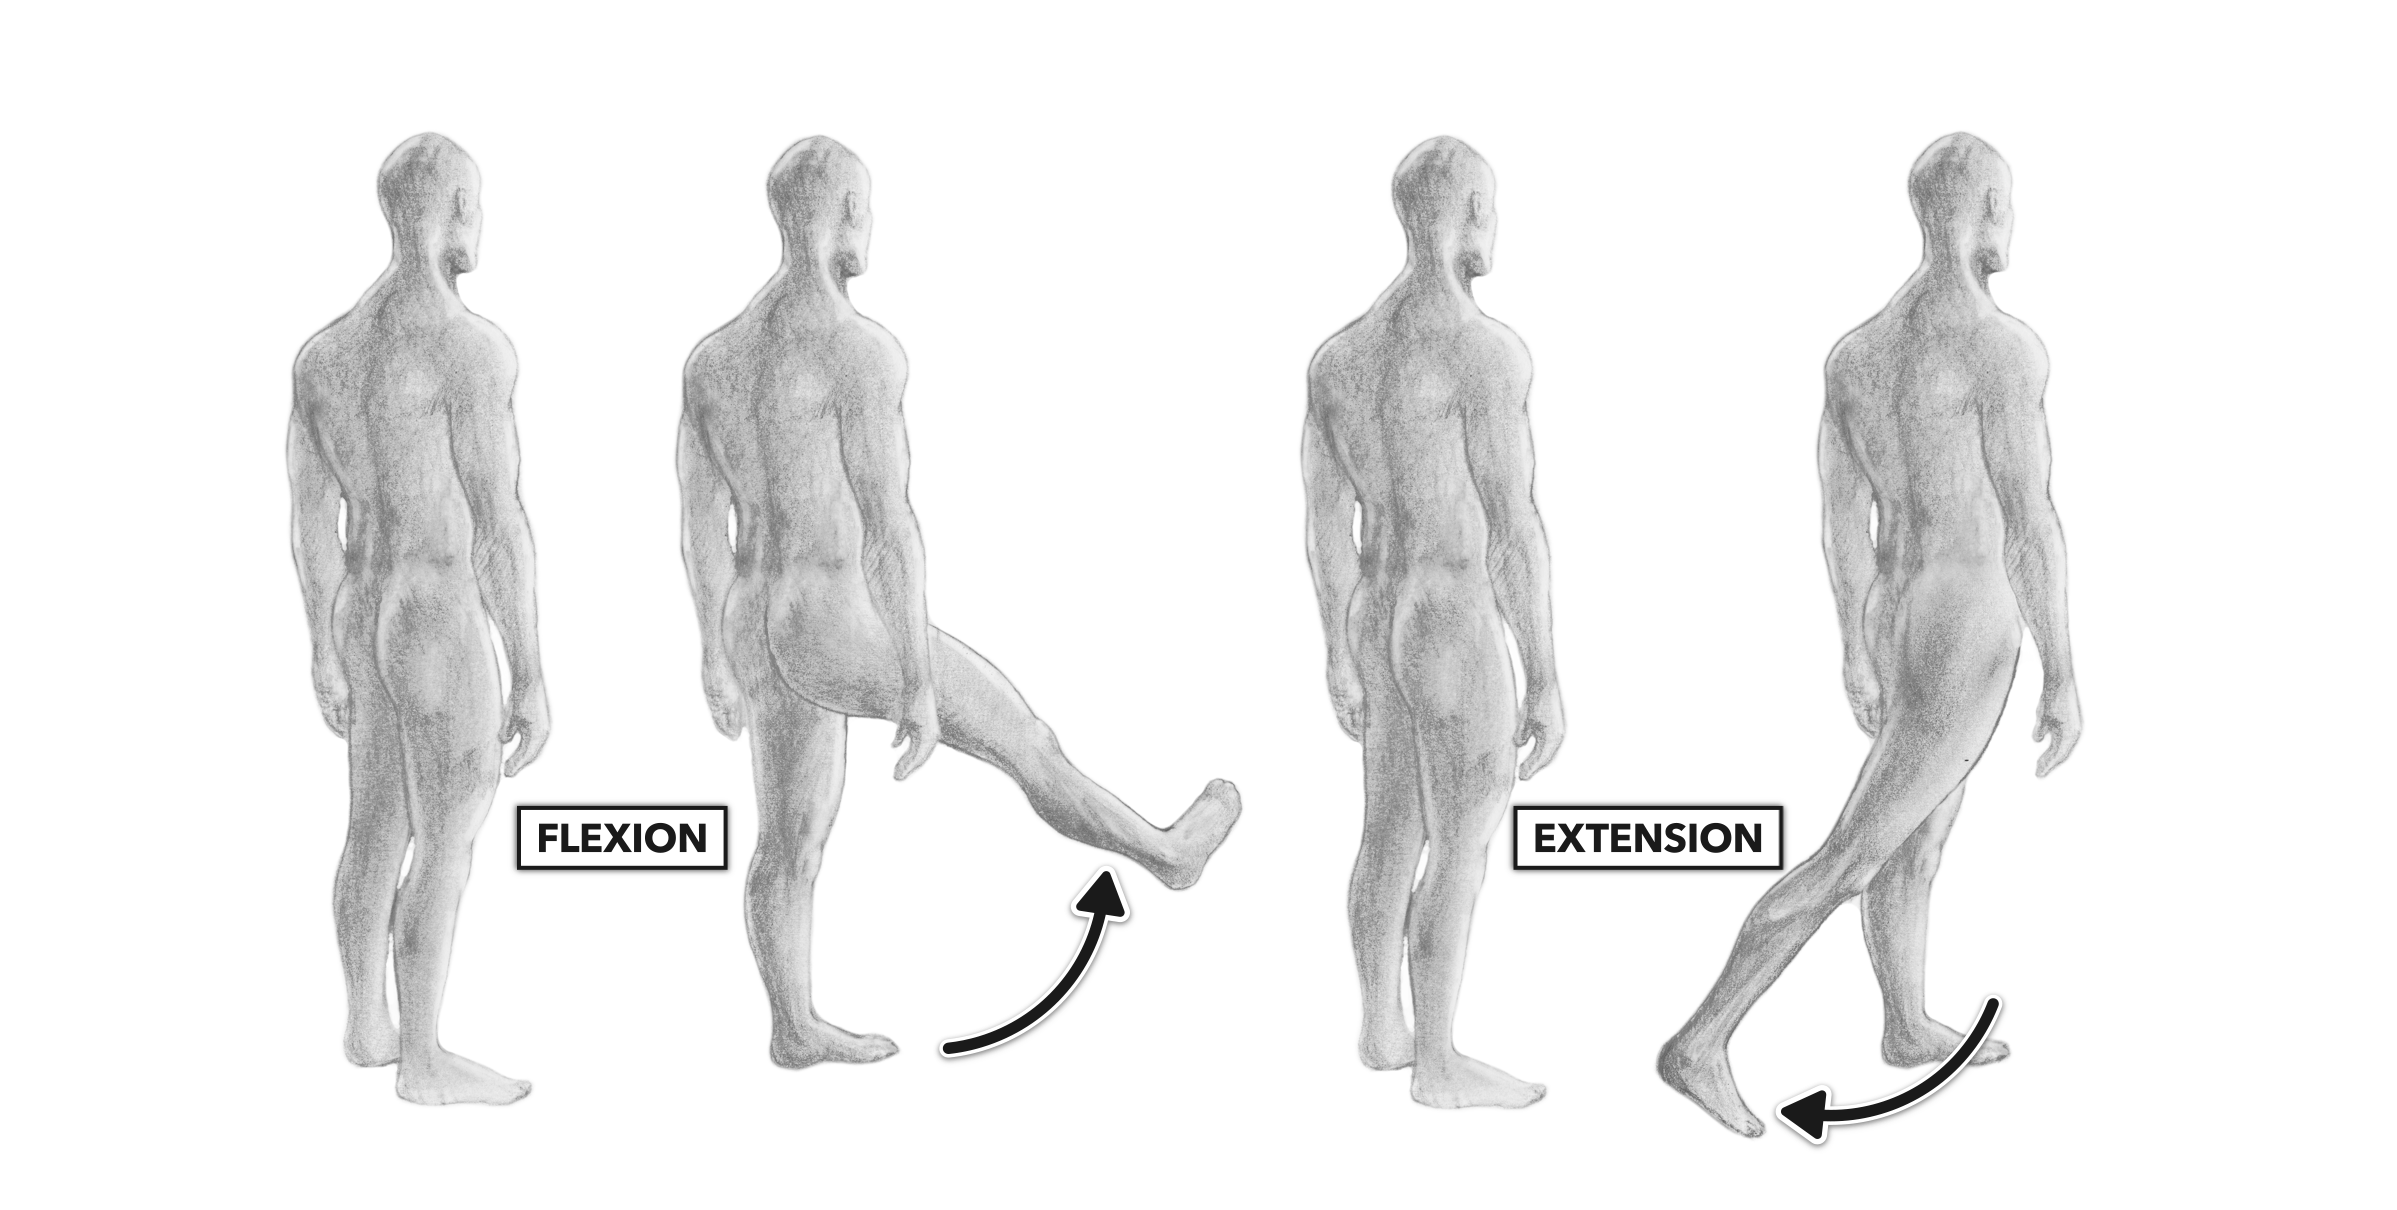
\includegraphics[width=\textwidth]{figures/hip.png}
    \caption{Afgebeeld de flexie en extensie van de heup. Afbeelding van https://www.crossfit.com/essentials/movement-about-joints-part-5-the-hip}
    \label{fig:hip}
\end{figure}

\begin{figure}[h]
    \centering
    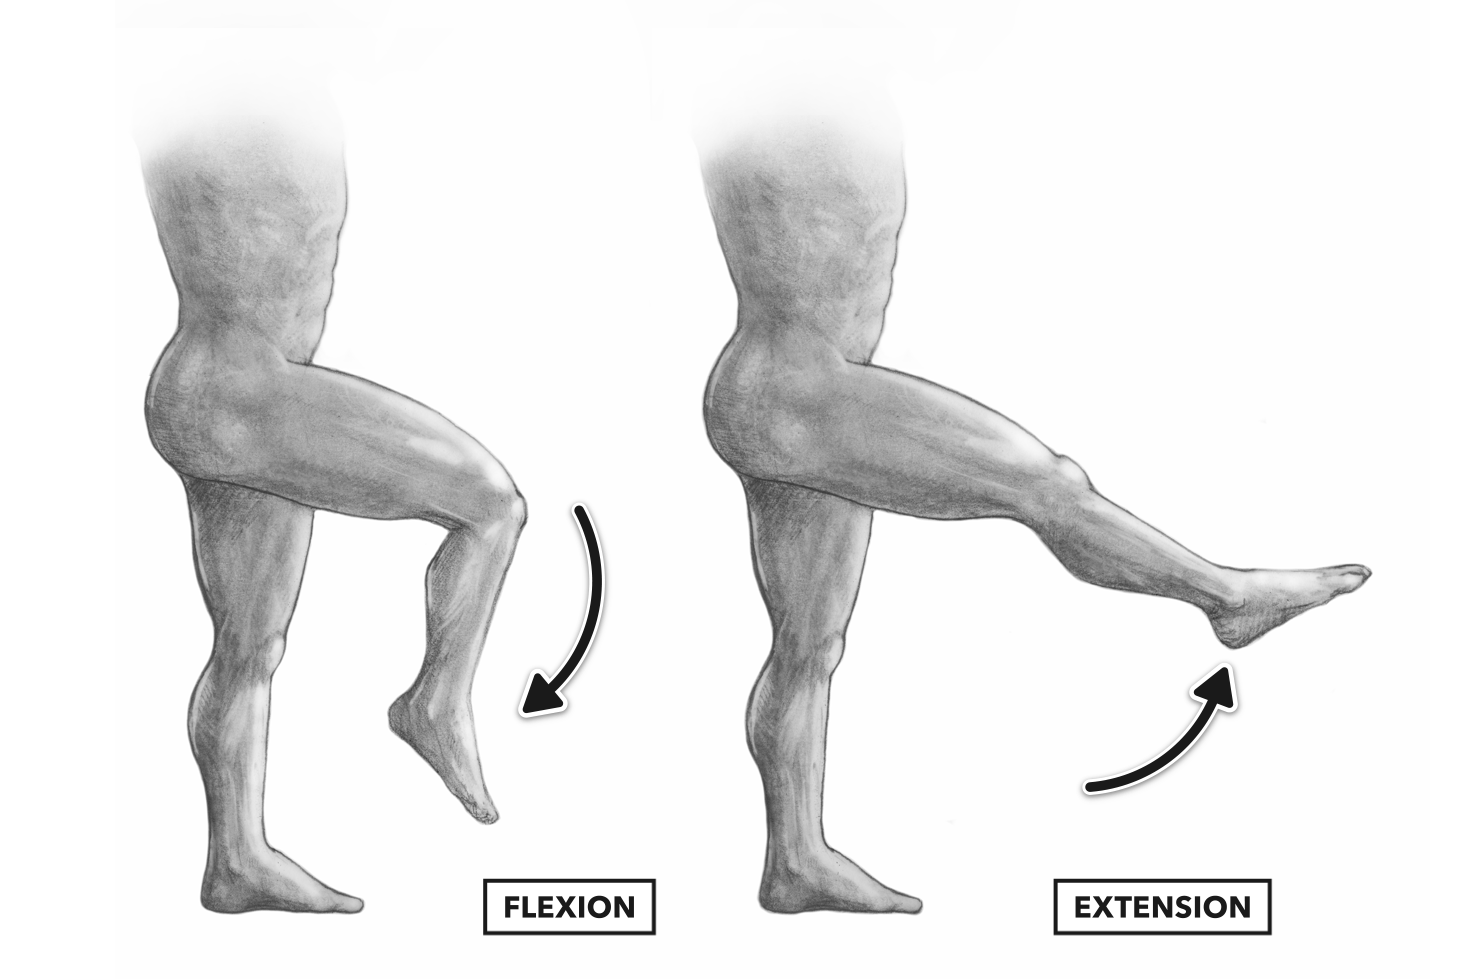
\includegraphics[width=\textwidth]{figures/knee.png}
    \caption{Afgebeeld de flexie en extensie van de knie. Afbeelding van https://www.crossfit.com/essentials/movement-about-joints-part-6-knee}
    \label{fig:knee}
\end{figure}

\begin{figure}[h]
    \centering
    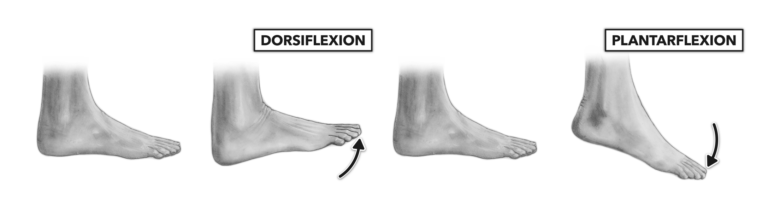
\includegraphics[width=\textwidth]{figures/ankle.png}
    \caption{Afgebeeld de flexie en extensie van de enkel, deze worden dorsiflexie en plantarflexie van de enkel genoemd. Dit verschilt van de normale flexie en extensie . Afbeelding van https://www.crossfit.com/essentials/movement-about-joints-part-7-the-ankle}
    \label{fig:ankle}
\end{figure}

\subsubsection{Opdracht 4}
De eerste opdracht over biomechanica! In deze opdracht zullen de studenten een schop uitvoeren, opnemen en analyseren. Er wordt kort geintroduceerd welke spieren en spiergroepen geactiveerd worden bij een schop, we zullen ook dit hier ook kort uitleggen. We zullen eerst het verschil tussen flexie (flexion) en extensie (extension) bespreken. Flexie wordt gedefinieerd als de buiging van gewrichten, waar extensie wordt gedefinieerd als het strekken vanuit de neutrale houding van gewrichten. In figuur \ref{fig:hip}, \ref{fig:knee} en \ref{fig:ankle} zijn respectievelijk de flexie en extensie van de heup, knie en enkel te zien. Om het (boven)been naar achter te trekken (heup extensie) worden de bilspieren geactiveerd, om het onderbeen naar achter te trekken (knie flexie) worden de hamstrings geactiveerd en om de voet naar achter te trekken (plantarflexie) wordt de gastrocnemius geactiveerd. In figuur \ref{fig:muscles} zijn de spieren die tijdens het eerste deel van de schop worden geactiveerd afgebeeld. Voor het tweede gedeelte van de schop zijn de spieren en spiergroepen in figuur \ref{fig:upper leg}. Om het bovenbeen naar voren te trekken (heup flexie) wordt iliopsoas geactiveerd en om het onderbeen naar voren te trekken (knie extensie) worden de quadriceps geactiveerd. \\\\

Nu we een beeld hebben van hoe de schop biomechanisch wordt uitgevoerd kunnen we kijken naar het analyseren van de beweging. Het is handig om de beweging te filmen in het donker, om zo nog een groter contrast te creëren. Als de data is verkregen, dit zijn dan de positie en hoeken van de gewrichten, kunnen de krachten die de spieren produceren worden berekend. Dit wordt gedaan met behulp van figuur 14 in de handleiding, waarin de spieren en de afstand tot het draaipunt wordt afgebeeld. De kracht van een spier wordt dan gegeven door,
\begin{align*}
    \tau &= Fr_\perp \\
    I\alpha &= Fr_\perp\\
    F &= \frac{I\alpha}{r_\perp}
\end{align*}
We zullen hier als voorbeeld de maximale spierkracht berekenen die door de quadriceps wordt gegenereerd. In figuur \ref{fig:schop} is de beweging van de schop te zien, met daarbij de hoek $\theta$ tussen het bovenbeen en onderbeen. De data van het filmpje wat opgenomen is, is te zien in figuur \ref{fig:hoek}. In figuur \ref{fig:hoekversnelling} is numeriek de tweede afgeleide bepaald. Dit is gedaan door eerst numeriek de eerste afgeleide te bepalen met behulp van het gemiddelde van Euler forward en Euler backward: 
\begin{align*}
    \dot{\theta}=\omega=\frac{\theta(t_{i-1}) - \theta(t_{i+1})}{\Delta t}
\end{align*}
voor een datapunt op tijdstip $t_i$, met $\Delta t=t_{i+1}-t_i$. Zie figuur \ref{fig:hoeksnelheid} voor de eerste numerieke afgeleide uitgezet tegen de tijd. Hiermee kan dan numeriek de tweede afgeleide worden bepaald:
\begin{align*}
    \ddot{\theta}=\alpha=\frac{\dot{\theta}(t_{i-1}) - \dot{\theta}(t_{i+1})}{\Delta t}.
\end{align*}
Om ruis te onderdrukken zijn de afgeleides bepaald van de ruwe data en van 3-punts gemmideldes,
\begin{align*}
    \theta_{avg}(t_i)=\frac{\theta(t_{i-1})+\theta(t_i)+\theta(t_{i+1})}{3}.
\end{align*}
In het algemeen kan er gekozen worden voor een $n$-punts gemmidelde, maar grotere $n$ hebben invloed op de data en daarmee ook op de afgeleides. We krijgen dan een maximale hoekversnelling van 5135.45 graden/s$^2=89.631$ rad/s$^2$ voor de gemiddelde data en 6768.36 graden/s$^2=118.13$ rad/s$^2$ voor de ongefilterde data. De kracht geleverd door de quadriceps is dan $F=\frac{0.20 \cdot 89.631}{0.04}=448.155$ N voor de gemiddelde data en $F=\frac{0.20 \cdot 118.13}{0.04}=590.65$ N voor de originele data, waarbij we een traagheidsmoment van het onderbeen hebben $I=0.2$ kgm$^{-2}$ gebruikt. De koppel is dan respectievelijk 17.9262 Nm en 23.626 Nm voor de gemiddelde en originele data. Als we dit vergelijken met de gemiddelde kracht die de quadriceps leveren, ongeveer 532 N (Force ratios in the quadriceps tendon and ligamentum patellae, Huberti et al.), zien we dat we er niet ver naast zitten. Wel moeten we bij deze vergelijking voorzichtig zijn, want het artikel waar de gemiddelde quadriceps kracht uit is gehaald heeft de kracht bepaald bij een specifieke beweging.

\subsection{Dagdeel 2}
Het tweede dagdeel zal vooral bedoeld zijn voor het verkennen en kiezen van een keuze-experiment, en het schrijven van een werkplan. Het kan zijn dat de verkenning van dagdeel 1 uitloopt tot dit dagdeel, maar deze uitloop moet tot een minimum gehouden worden omdat bij dit experiment de uitvoering van de experimenten vrij lang kan duren. Er kan gekozen worden voor een biomechanisch of een klassiek mechanisch experiment. Belangrijk is dat de studenten tijdens dit dagdeel al goed duidelijk hebben wat ze willen bepalen, of hier een model/theorie voor is en of het experiment haalbaar is, bespreek dit ook met de stafleden. \\\\ Het is vooral bij dit experiment belangrijk dat de studenten goed nadenken over hun keuze-experiment voordat ze deze gaan uitvoeren. Dit betekent dat het werkplan zoveel mogelijk een complete theorie en methode moet bevatten. Het is op zich niet erg als deze niet helemaal correct of compleet zijn, maar pas wel op dat de student niet in tijdsnood komt omdat het niet duidelijk is wat er gedaan moet worden.

\subsection{Dagdeel 3}
Het eerste dagdeel waar de studenten zullen beginnen met hun keuze-experimenten. Dit dagdeel begint dan met een korte introductie en het bespreken van de werkplannen. In dit dagdeel zullen de koppels studenten de werkplannen laten presenteren onder begeleiden van de assistent. De presentaties worden dan van feedback voorzien door de assistent en de medestudenten. Het is sterk aangeraden dat de studenten de opstelling bouwen, 1 meetserie doen en deze vervolgens helemaal gaan analyseren. Zo hebben ze een keer de stappen in hun werkplan doorgewerkt en gecontroleerd of hun theorie en methode kloppen.

\subsection{Dagdeel 4 en verder}
In de komende dagdelen zullen studenten verder werken aan hun experiment en de data analyseren die ze tijdens deze dagdelen hebben verkregen. Het zou voor de studenten die een biomechanisch experiment doen erg nuttig zijn om bronnen te vinden waarmee ze hun data kunnen vergelijken. Het zou optimaal zijn als dit al is uitgezocht in het werkplan, maar het is ook mogelijk om dit in de later dagdelen uit te zoeken mits daar tijd voor is. 


\begin{figure}[h]
    \centering
    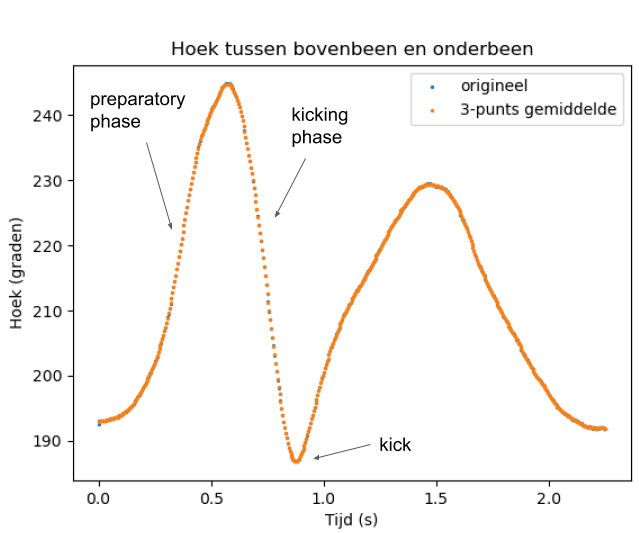
\includegraphics[width=\textwidth]{figures/Figure_1.png}
    \caption{De hoek, zoals gedefinieerd in figuur \ref{fig:schop}, uitgezet tegen te tijd. Van de data is het origineel en de 3-punts gemiddelde geplot, en deze zijn vrijwel hetzelfde.}
    \label{fig:hoek}
\end{figure}

\begin{figure}[h]
    \centering
    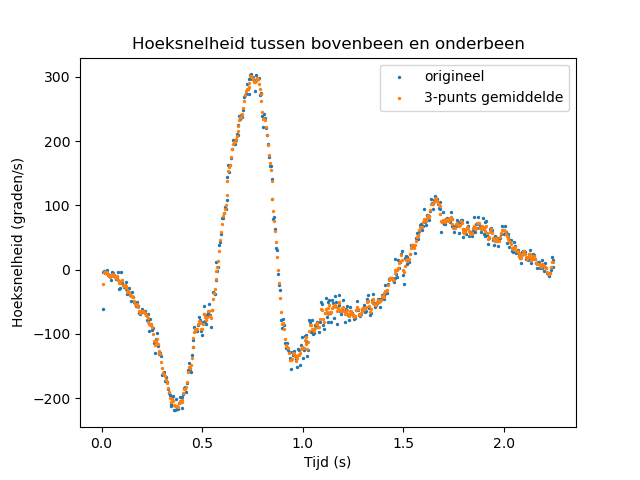
\includegraphics[width=\textwidth]{figures/Figure_2.png}
    \caption{Hier is van de ruwe data van figuur \ref{fig:hoek} de numerieke eerste afgeleide berekend door het gemiddelde van Euler forward en backward te nemen: $\dot{\theta}=\omega=\frac{\theta(t_{i-1}) - \theta(t_{i+1})}{\Delta t}$. We zien al dat het signaal sporen bevat van hoogfrequent signaal, maar dit nog enigszins te onderdrukken valt door de data te middelen.}
    \label{fig:hoeksnelheid}
\end{figure}

\begin{figure}[h]
    \centering
    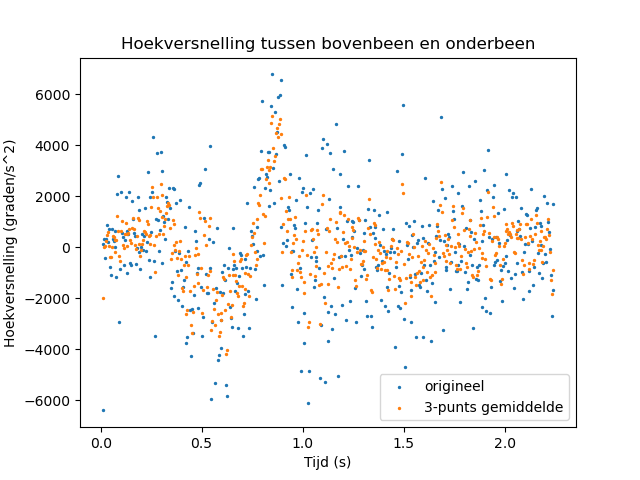
\includegraphics[width=\textwidth]{figures/hoekversnelling.png}
    \caption{De hoekversnelling is hier berekend met behulp van dezelfde methode: gemiddelde van Euler forward en backward. We zien dat het signaal wordt gedomineerd door hoogfrequente ruis, wat een gevolg is van de methode die we gebruiken om de afgeleide en tweede afgeleide te berekenen. We kunnen de maximum voor zowel het gemiddelde signaal als het originele (ongefilterde) signaal bepalen, deze zijn respectievelijk 5135,45 graden/s$^2$ en 6768,36 graden/s$^2$}
    \label{fig:hoekversnelling}
\end{figure}

\begin{figure}[h]
    \centering
    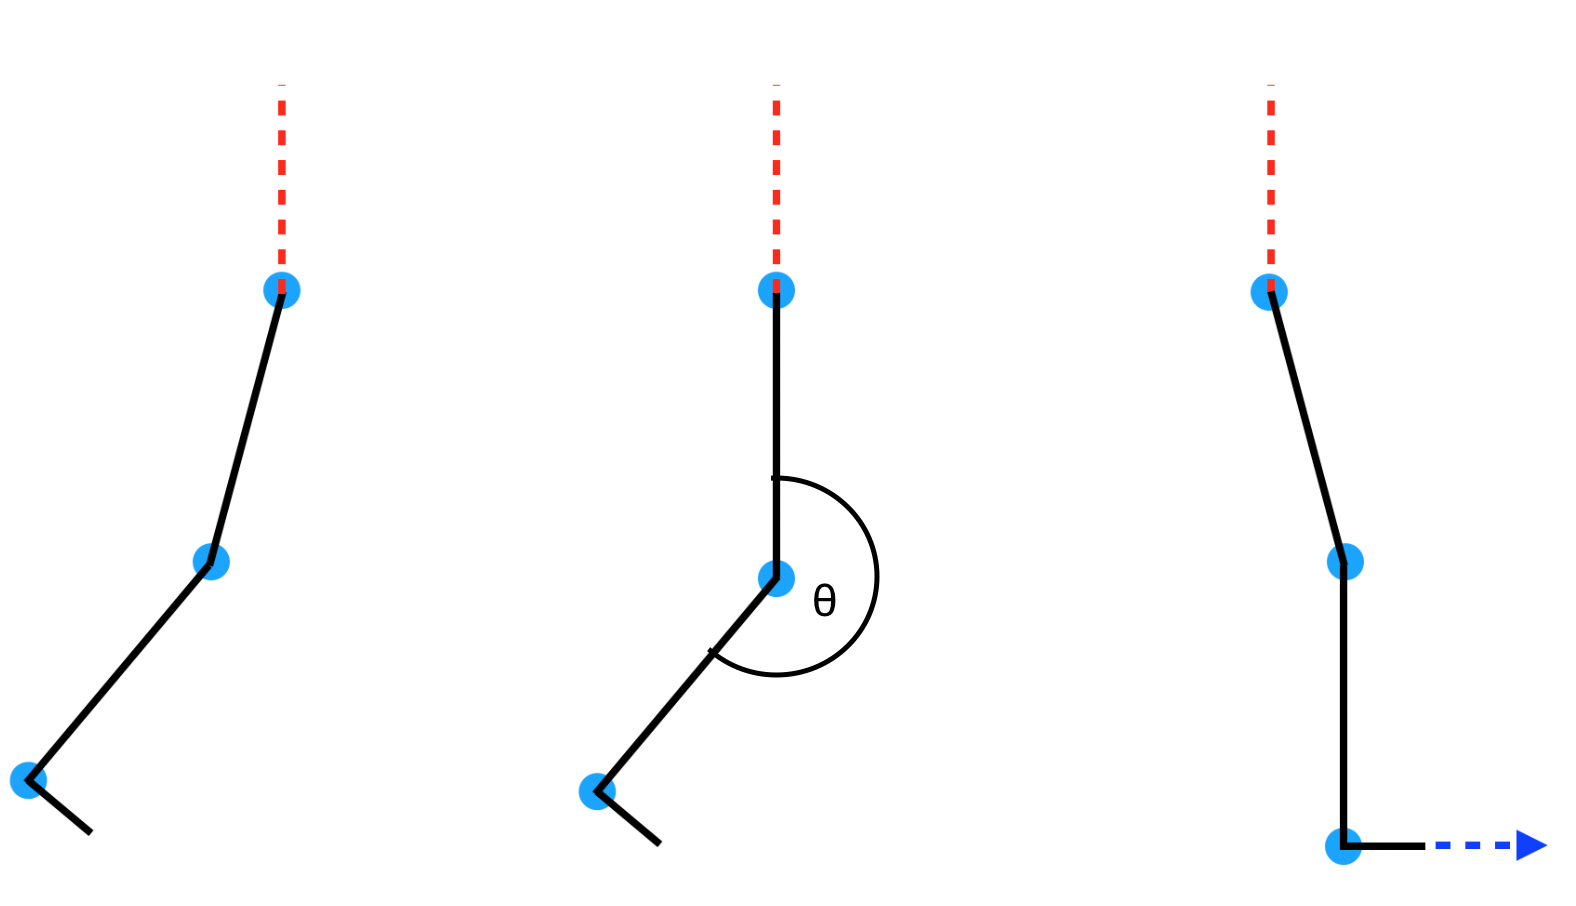
\includegraphics[width=\textwidth]{figures/schop.png}
    \caption{De beweging van de schop die van links naar rechts wordt uitgevoerd. Ook is de hoek tussen de bovenbeen en onderbeen $\theta$ te zien.}
    \label{fig:schop}
\end{figure}

\begin{figure}
    \centering
    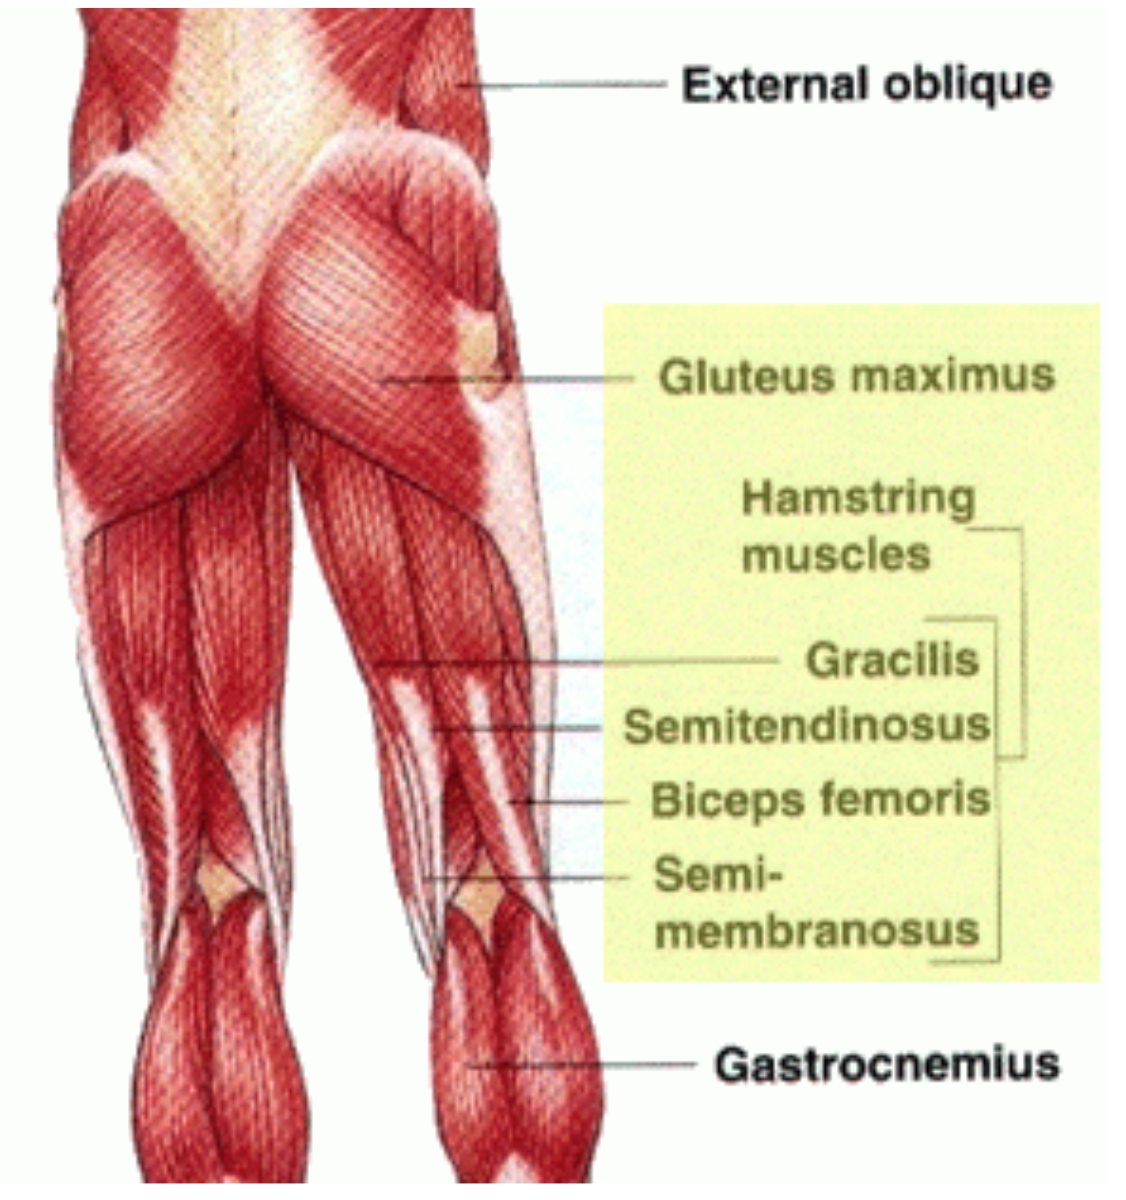
\includegraphics[width=\textwidth]{figures/muscles.png}
    \caption{Afgebeeld de spieren en spiergroepen van de achterkant van het been. Afbeelding van https://equilibriumsas.com.au/can-weak-gluteals-cause-back-pain/}
    \label{fig:muscles}
\end{figure}

\begin{figure}
    \centering
    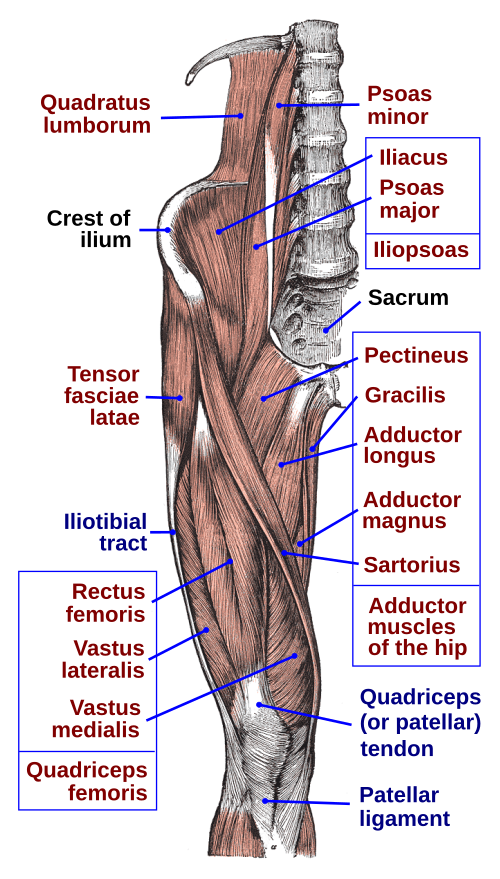
\includegraphics[width=0.6\textwidth]{figures/upper leg.png}
    \caption{Afgebeeld de spieren en spiergroepen van de voorkant van het been. Hierbij zijn de belangrijkste spiergroepen de iliopsoas en quadriceps. Afbeelding van https://en.wikipedia.org/wiki/Iliopsoas}
    \label{fig:upper leg}
\end{figure}

\end{document}
